\section{Sheaf Cobordism on Generator Regions}
Suppose we have a punctured Riemann sphere $M$ and $\Lambda_0^0$, $\Lambda_0^\infty$, $\Lambda_0^{squig}$, a nested regions $U\subset U' \subset M$, and a chart $f : U \rightarrow \R^2$ such that $U'$ maps to $R:=(-1,1)_x \times (-n-1,n+1)_z$ under $f$
\begin{itemize}
\item $\Lambda_0^0$ gets mapped to the red strands in the figure below, co-oriented upward.

\item $\Lambda_0^\infty$ gets mapped to the blue strands in the figure below, co-oriented downward.

\item $\Lambda_0^{squig}$ gets mapped to the squiggly lines with co-orientations given in the figure below.
\end{itemize}
and a sheaf defined by the following squiggly legible diagram. All the maps corresponding to blue strands are $\iota_1$ and the red strands $\iota_0$ otherwise stated. I have omitted these maps from the diagram.\\

\begin{figure}[H]
    \centering
    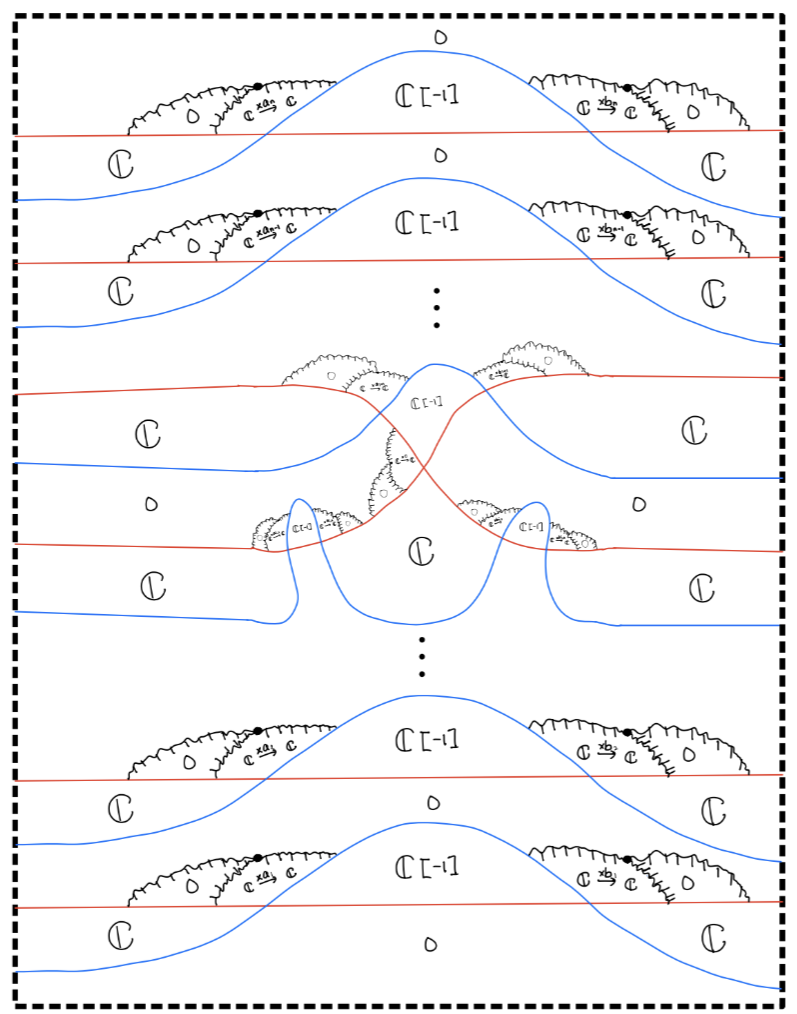
\includegraphics[scale = 0.95]{diagrams/cobord_gen/1.png}
    \caption{}
    \label{fig:your-label}
\end{figure}

Then we define a cobordism starting from the above sheaf, say $cobord_{gen}(n)$ supported on $U$, where $n$ is the number of blue strands(equivalently, red strands). At the end of the cobordism, the sheaf, under the same chart $f$, is described as the following squiggly legible diagram. 
\begin{figure}[H]
    \centering
    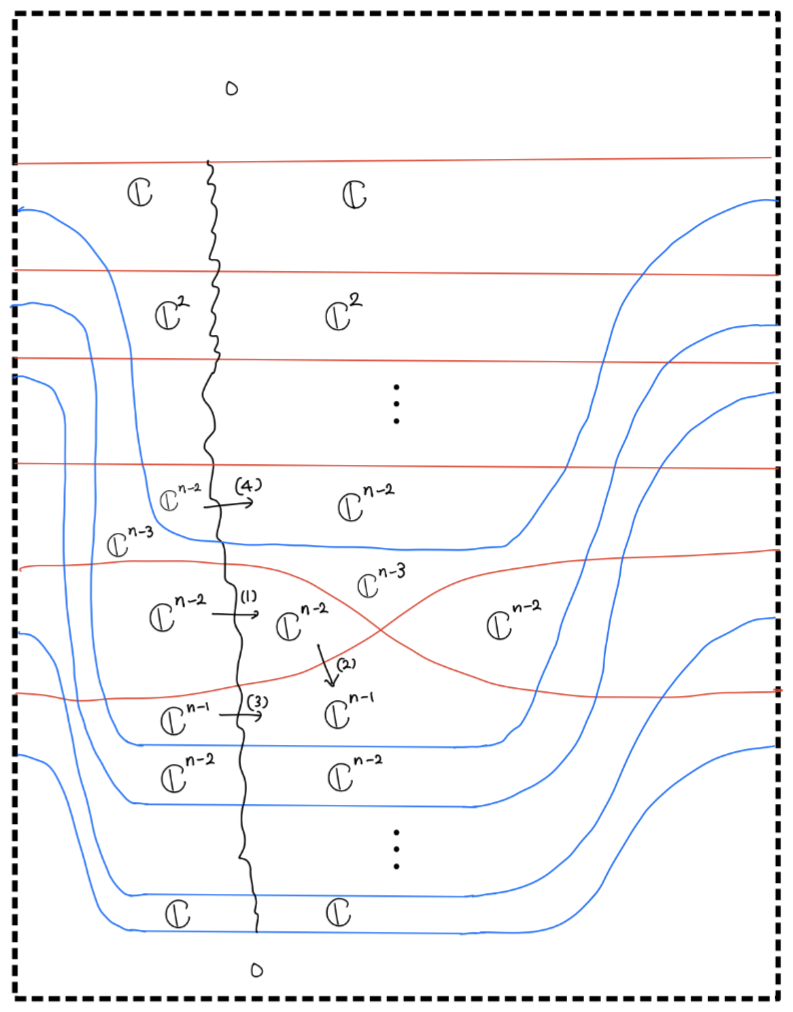
\includegraphics[scale = 0.95]{diagrams/cobord_gen/15.png}
    \caption{}
    \label{fig:your-label}
\end{figure}
\pagebreak
\textbf{Generization maps}
\begin{enumerate}[label = (\arabic*)]
\item $diag(d_n,\cdots,d_{i+1})$

\item $\iota_0 \circ diag(1,\cdots,1) + e' I_{n-i+1,n-i}$

\item $diag(d_n,\cdots,d_{i+1}) + e I_{n-i+1,n-i}$
\end{enumerate}
where
\begin{itemize}
\item $d_r = a_r b_r^{-1}$
\item $e = -a_{i+1}b_i^{-1}c$
\item $e' = d_{i+1}^{-1}e$
\end{itemize}
\pagebreak
We define $cobord_{gen}(n)$ inductively as follows.
\begin{enumerate}[label = (\roman*)]
\item For $n=2$, we define $cobord_{gen}$ starting from the sheaf below
\begin{figure}[H]
    \centering
    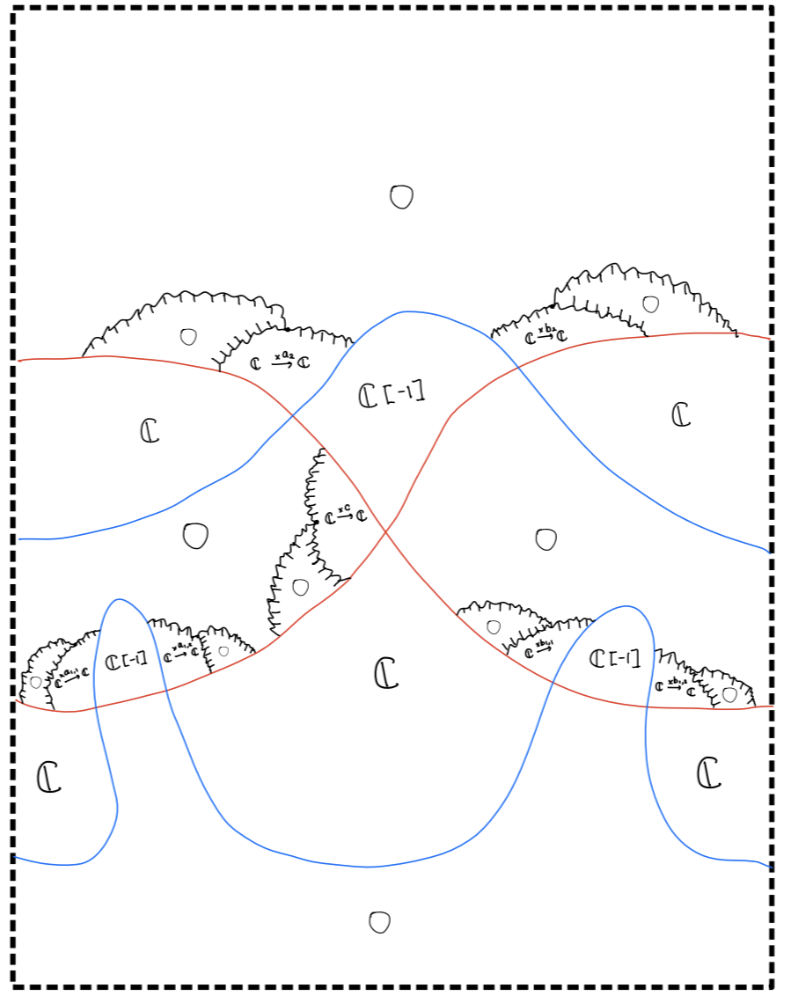
\includegraphics[scale = 0.95]{diagrams/cobord_gen/base_1.png}
    \caption{}
    \label{fig:your-label}
\end{figure}
as follows.
\pagebreak
\begin{enumerate}[label = (Step \arabic*)]
\item we apply $cobord_1$ to the square regions surrounded by purple dotted lines.
\begin{figure}[H]
    \centering
    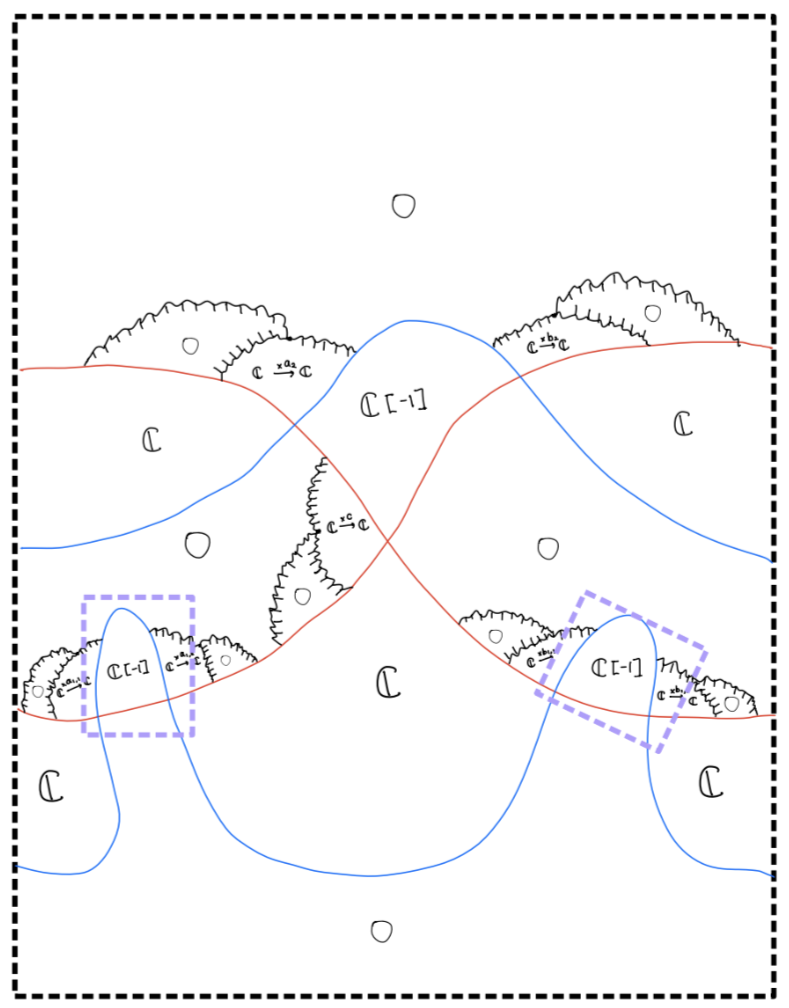
\includegraphics[scale = 0.95]{diagrams/cobord_gen/base_2.png}
    \caption{}
    \label{fig:your-label}
\end{figure}
\pagebreak
we get
\begin{figure}[H]
    \centering
    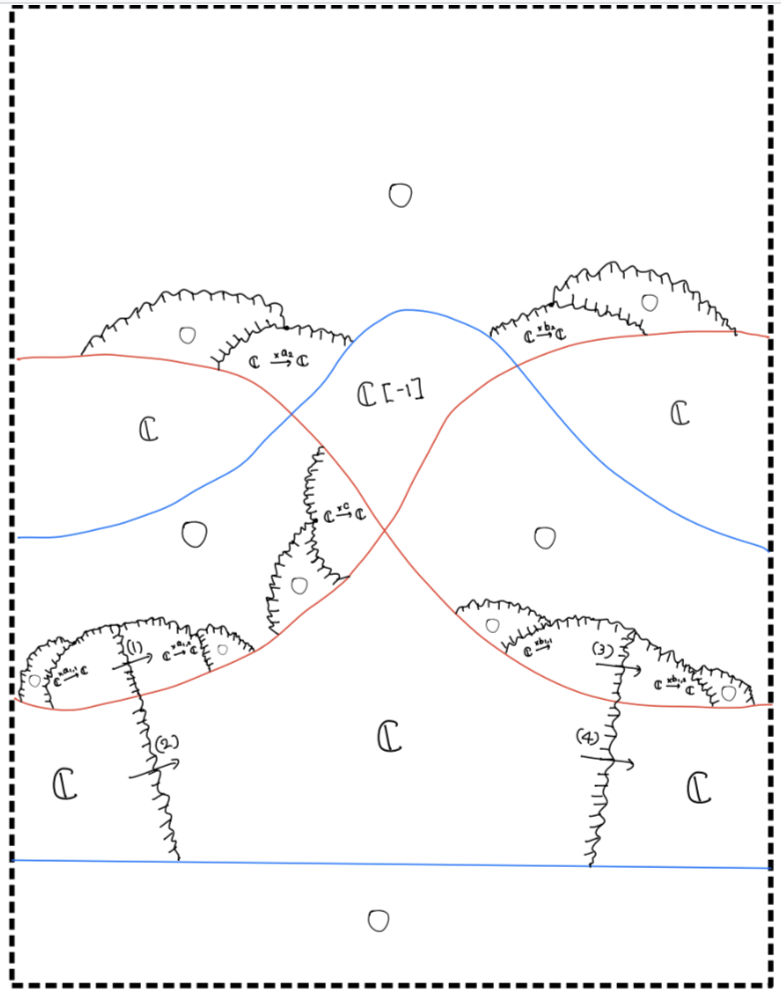
\includegraphics[scale = 0.95]{diagrams/cobord_gen/base_3.png}
    \caption{}
    \label{fig:your-label}
\end{figure}
\pagebreak
\textbf{Generization maps}
\begin{enumerate}[label = (\arabic*)]
\item 
\begin{tikzcd}
\C \arrow[r, "\times 1"] & \C \\
\C \arrow[r, "\times a_{1,1}"]\arrow[u, "\times a_1"] & \C \arrow[u, "\times a_{1,2}"]
\end{tikzcd}

\item $\times a_1$

\item 
\begin{tikzcd}
\C \arrow[r, "\times 1"] & \C \\
\C \arrow[r, "\times b_{1,1}"]\arrow[u, "\times b_1^{-1}"] & \C \arrow[u, "\times b_{1,2}"]
\end{tikzcd}

\item $\times b_1^{-1}$
\end{enumerate}
where
\begin{itemize}
\item $a_1 = a_{1,1}a_{1,2}^{-1}$
\item $b_1 = b_{1,1}^{-1}b_{1,2}$
\end{itemize}
\pagebreak
which is quasi-isomorphic to
\begin{figure}[H]
    \centering
    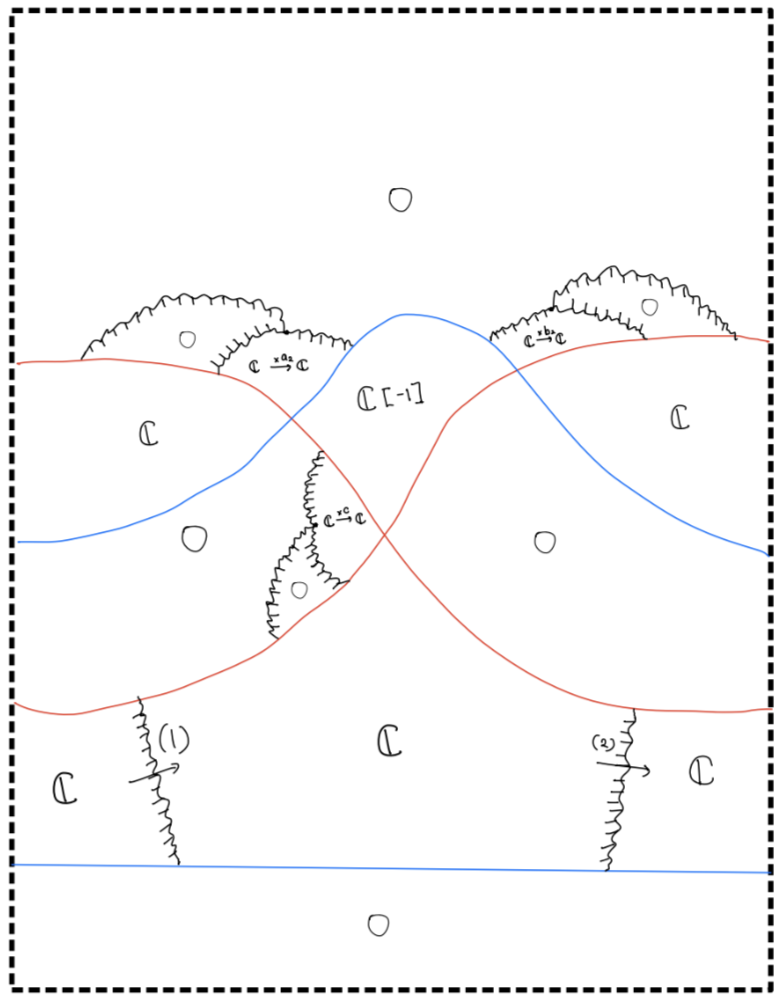
\includegraphics[scale = 0.95]{diagrams/cobord_gen/base_4.png}
    \caption{}
    \label{fig:your-label}
\end{figure}
\textbf{Generization maps}
\begin{enumerate}[label = (\arabic*)]
\item $\times a_1$

\item $\times b_1^{-1}$
\end{enumerate}
\pagebreak
\item apply $cobord_8$ to the region surrounded by a purple dotted line
\begin{figure}[H]
    \centering
    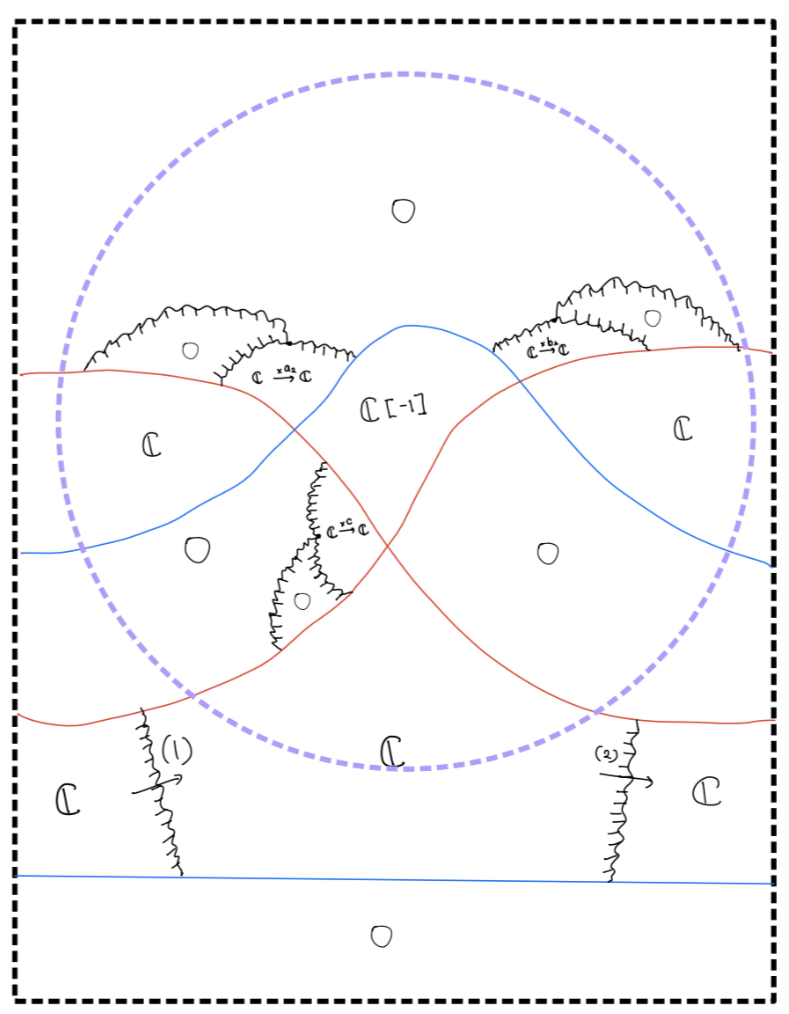
\includegraphics[scale = 0.95]{diagrams/cobord_gen/base_5.png}
    \caption{}
    \label{fig:your-label}
\end{figure}
\pagebreak
we get
\begin{figure}[H]
    \centering
    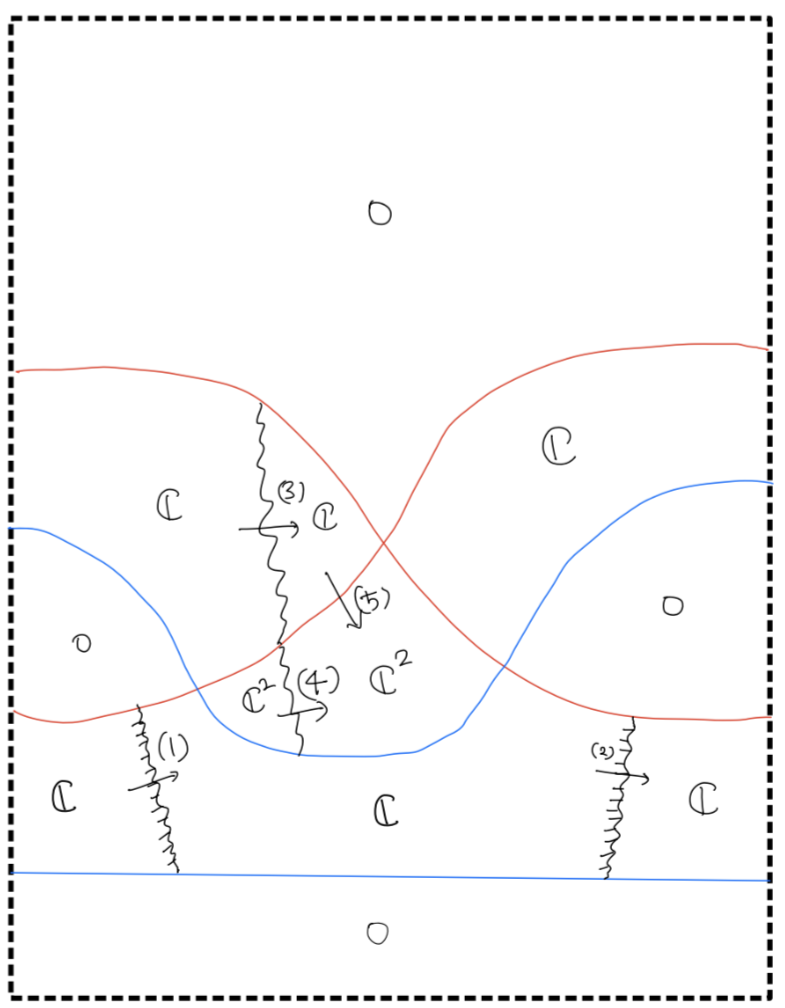
\includegraphics[scale = 0.95]{diagrams/cobord_gen/base_6.png}
    \caption{}
    \label{fig:your-label}
\end{figure}
\pagebreak
\textbf{Generization maps}
\begin{enumerate}[label = (\arabic*)]
\item $\times a_1$

\item $\times b_1^{-1}$

\item $\times a_2b_2^{-1}$

\item 
$\begin{pmatrix}
a_2b_2^{-1} & 0 \\
-a_2c^{-1} & 1
\end{pmatrix}$

\item 
$\begin{pmatrix}
1 \\
-b_2c^{-1} 
\end{pmatrix}$
\end{enumerate}

\pagebreak
which is quasi-isomorphic to
\begin{figure}[H]
    \centering
    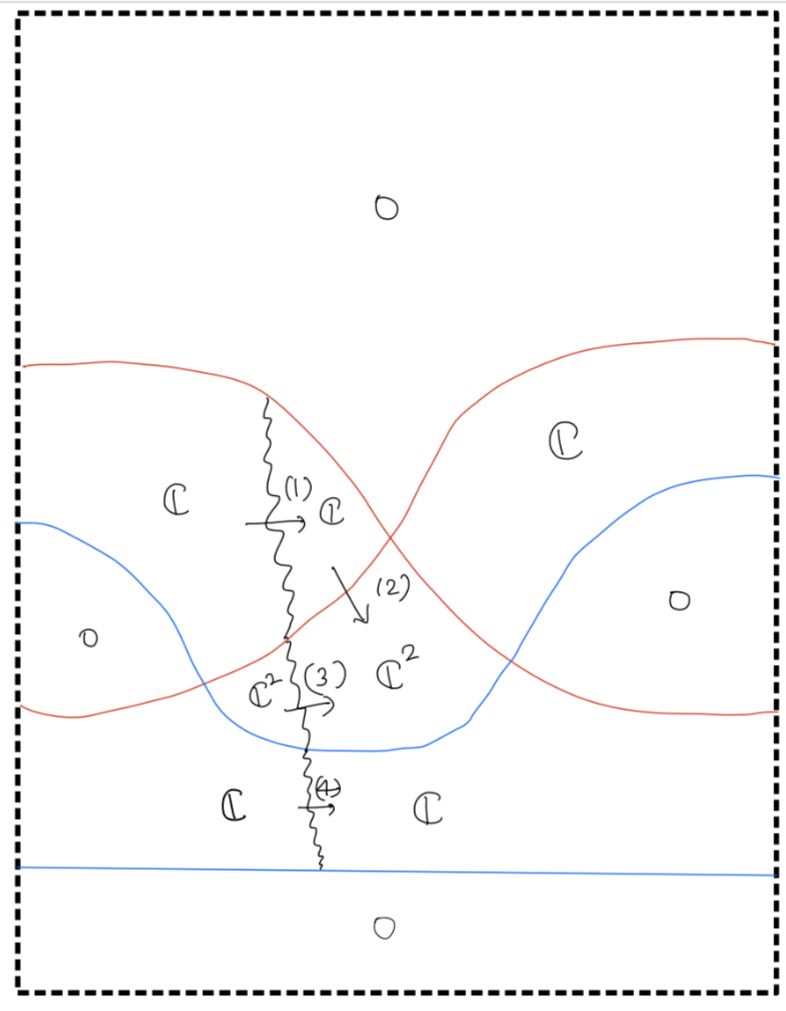
\includegraphics[scale = 0.95]{diagrams/cobord_gen/base_7.png}
    \caption{}
    \label{fig:your-label}
\end{figure}
\pagebreak
\textbf{Generization maps}
\begin{enumerate}[label = (\arabic*)]
\item $\times d_2$

\item 
$\begin{pmatrix}
1 \\
e' 
\end{pmatrix}$

\item 
$\begin{pmatrix}
d_2 & 0 \\
e & d_1
\end{pmatrix}$

\item $\times d_1$
\end{enumerate}
where
\begin{itemize}
\item $d_r = a_rb_r^{-1}$
\item $e = -a_2b_1^{-1}c$
\item $e' = d_2^{-1}e$
\end{itemize}
\end{enumerate}
\pagebreak
\item For $n>2$,
\begin{enumerate}[label = (Case \arabic*)]
\item if the generator $s_i$ is $i\neq 1$,
\begin{enumerate}[label = (Step \arabic*)]
\item we apply $cobord_{gen}(n-1)$ to the square region surrounded by purple dotted lines.

\begin{figure}[H]
    \centering
    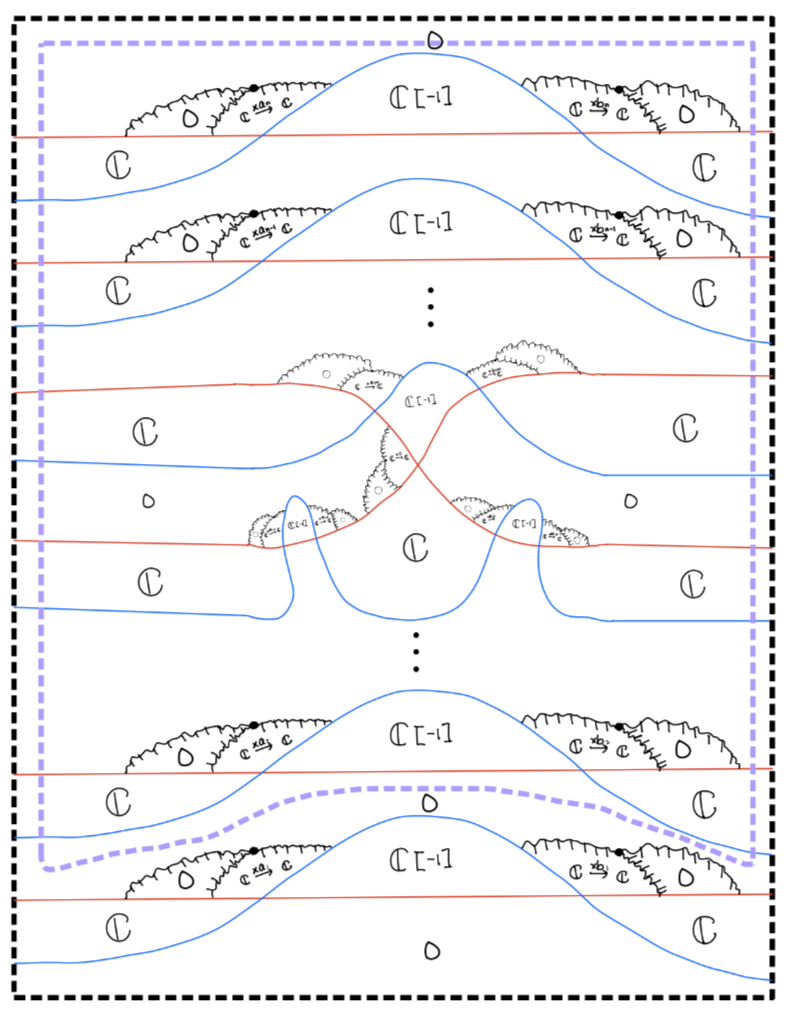
\includegraphics[scale = 0.95]{diagrams/cobord_gen/2.png}
    \caption{}
    \label{fig:your-label}
\end{figure}
\pagebreak
by induction hypothesis, we get

\begin{figure}[H]
    \centering
    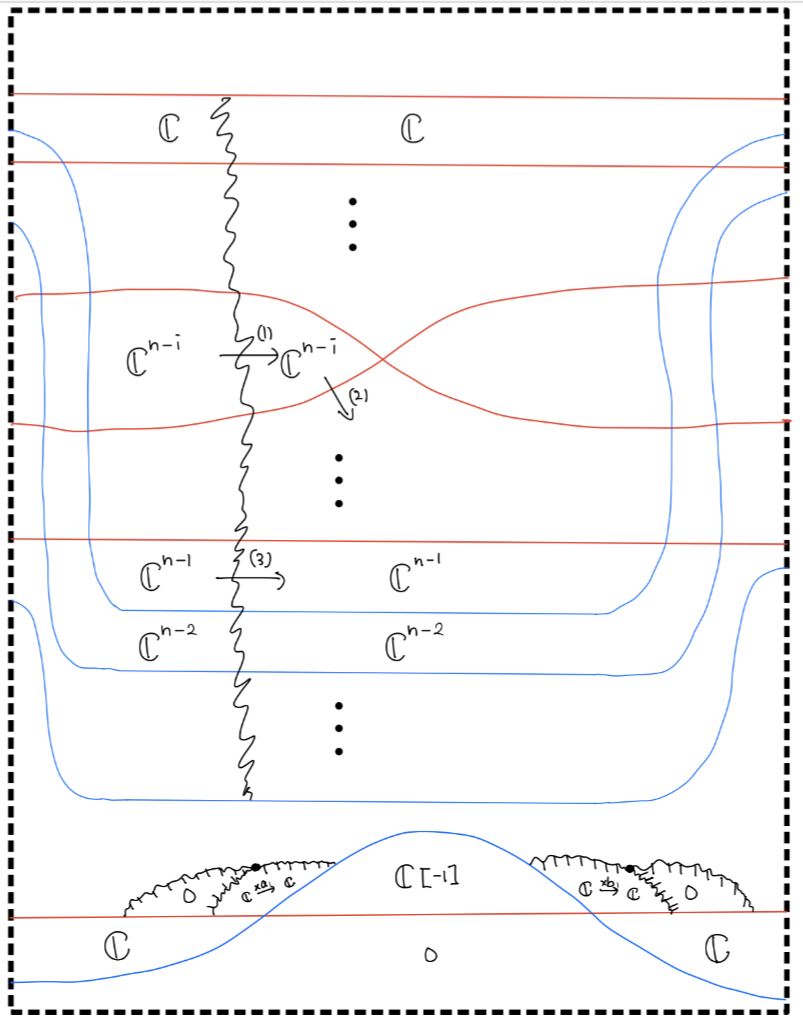
\includegraphics[scale = 0.95]{diagrams/cobord_gen/3.png}
    \caption{}
    \label{fig:your-label}
\end{figure}
\textbf{Generization maps}
\begin{enumerate}[label = (\arabic*)]
\item $diag(d_n,\cdots,d_{i+1})$
\item $\iota_0 \circ diag(1,\cdots,1) + e' I_{n-i+1,n-i}$
\item $diag(d_n,\cdots,d_2) + e I_{n-i+1,n-i}$
\end{enumerate}
\pagebreak
\item apply $cobord_2$ to the region surrounded by a purple dotted line.

\begin{figure}[H]
    \centering
    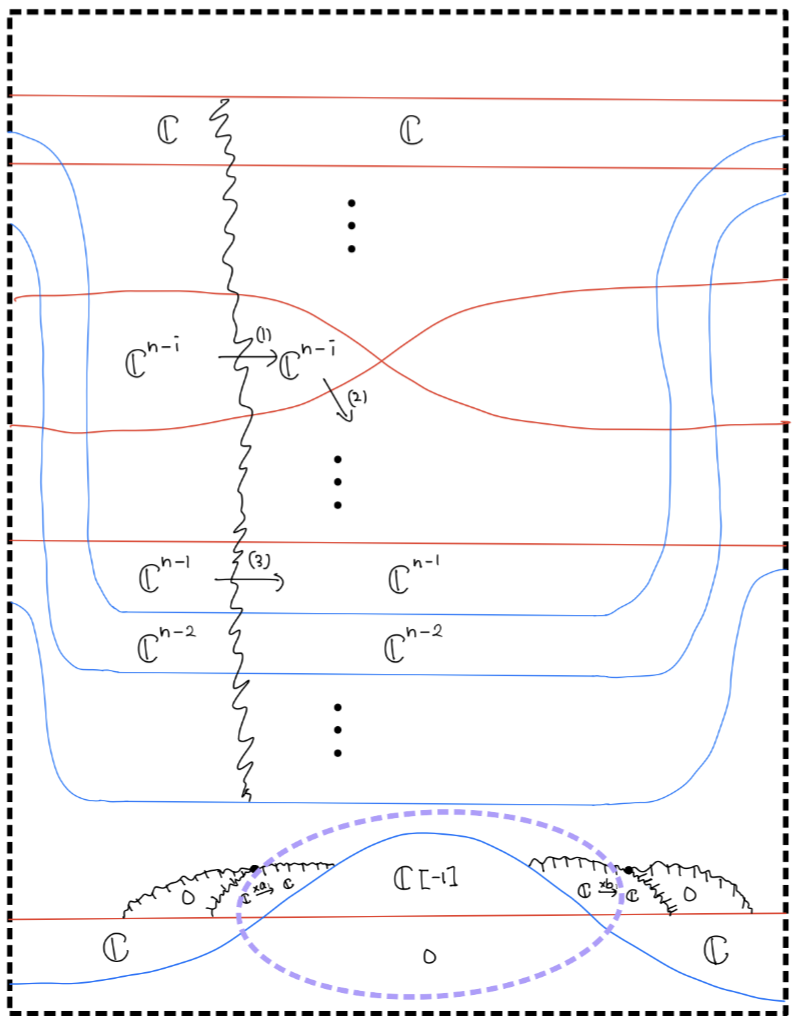
\includegraphics[scale = 0.95]{diagrams/cobord_gen/4.png}
    \caption{}
    \label{fig:your-label}
\end{figure}
\pagebreak
we get

\begin{figure}[H]
    \centering
    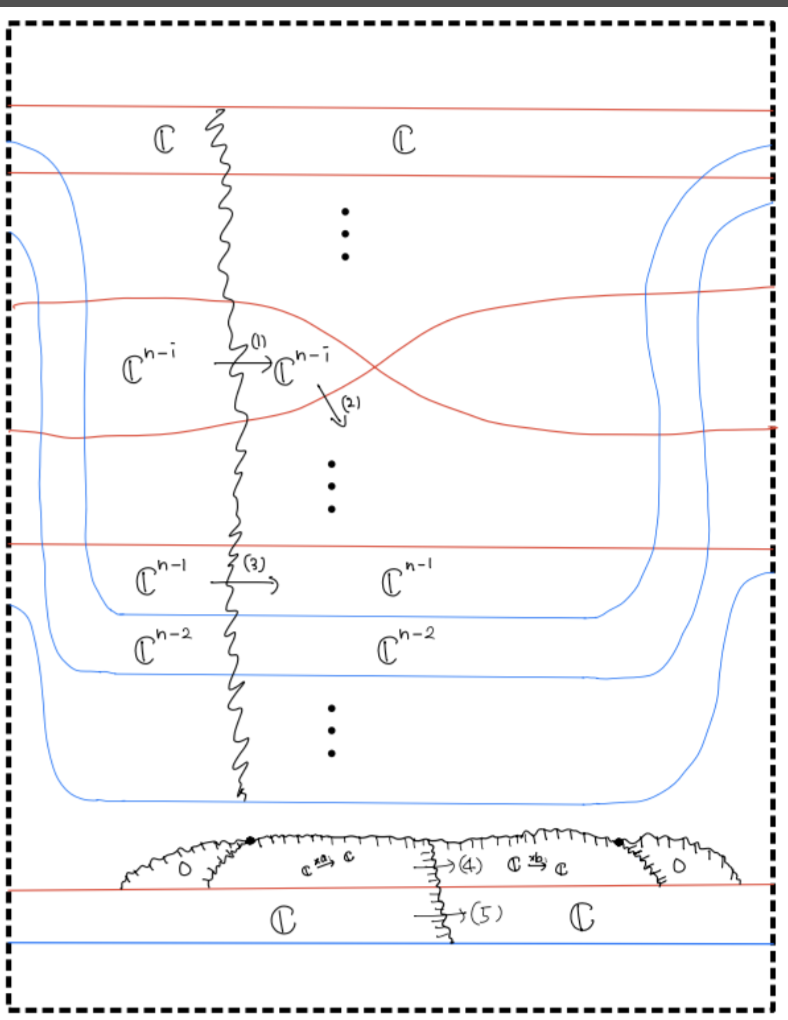
\includegraphics[scale = 0.95]{diagrams/cobord_gen/5.png}
    \caption{}
    \label{fig:your-label}
\end{figure}
\pagebreak
\textbf{Generization maps}
\begin{enumerate}[label = (\arabic*)]
\item $diag(d_n,\cdots,d_{i+1})$
\item $\iota_0 \circ diag(1,\cdots,1) + e' I_{n-i+1,n-i}$
\item $diag(d_n,\cdots,d_2) + e I_{n-i+1,n-i}$
\item 
\begin{tikzcd}
\C \arrow[r,"\times 1"] & \C\\
\C \arrow[r,"\times d_1"]\arrow[u,"\times a_1"] & \C\arrow[u,"\times b_1"]
\end{tikzcd}
\item $\times d_1$ 
\end{enumerate}
\pagebreak
which is quasi-isomorphic to 

\begin{figure}[H]
    \centering
    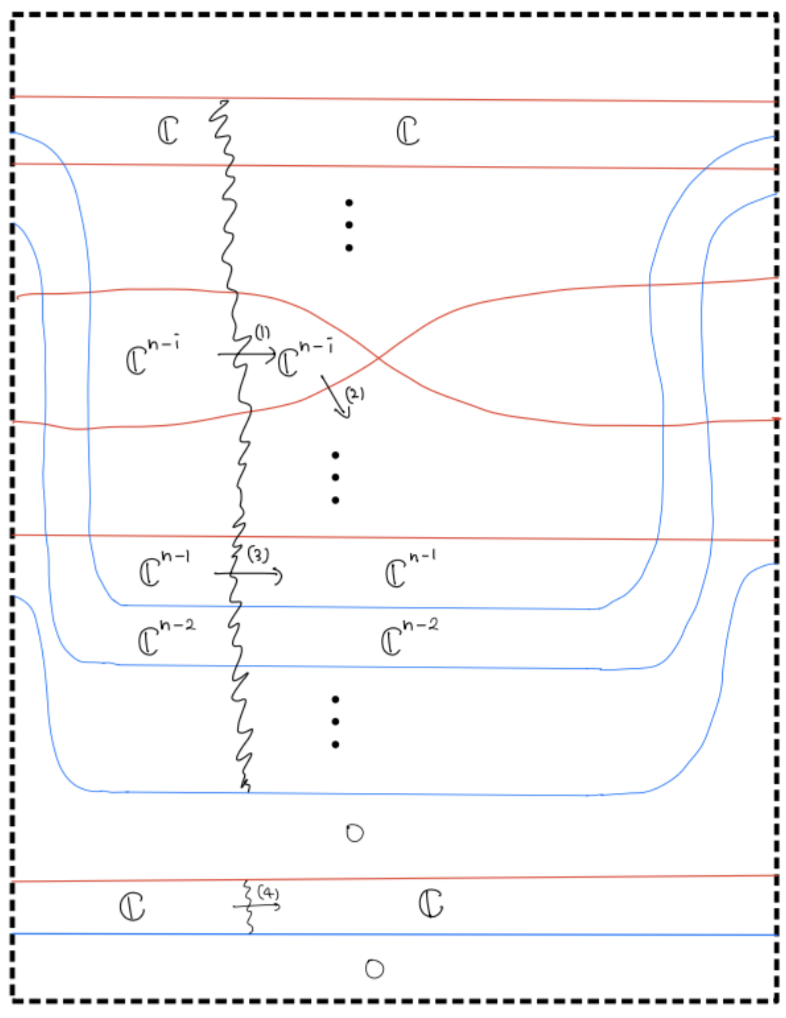
\includegraphics[scale = 0.85]{diagrams/cobord_gen/6.png}
    \caption{}
    \label{fig:your-label}
\end{figure}
\textbf{Generization maps}
\begin{enumerate}[label = (\arabic*)]
\item $diag(d_n,\cdots,d_{i+1})$
\item $\iota_0 \circ diag(1,\cdots,1) + e' I_{n-i+1,n-i}$
\item $diag(d_n,\cdots,d_2) + e I_{n-i+1,n-i}$
\item $\times d_1$ 
\end{enumerate}
\pagebreak
\item apply $cobord_6$ to the square region surrounded by purple dotted lines.

\begin{figure}[H]
    \centering
    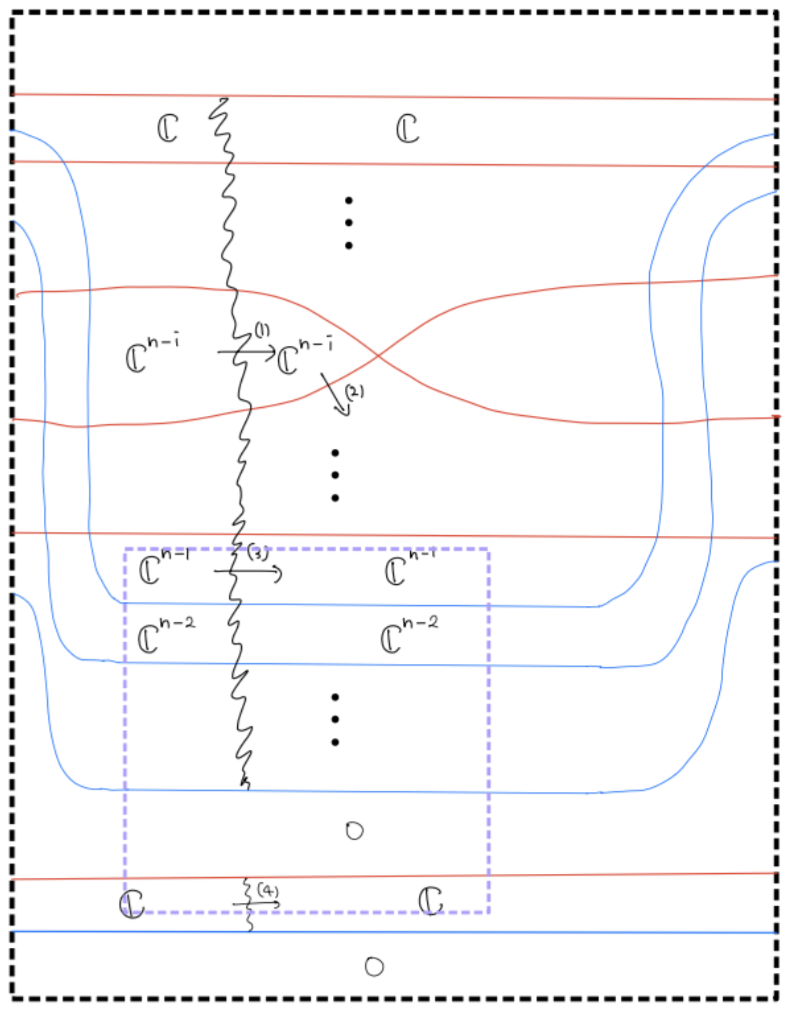
\includegraphics[scale = 0.95]{diagrams/cobord_gen/7.png}
    \caption{}
    \label{fig:your-label}
\end{figure}
\pagebreak
we get the final sheaf

\begin{figure}[H]
    \centering
    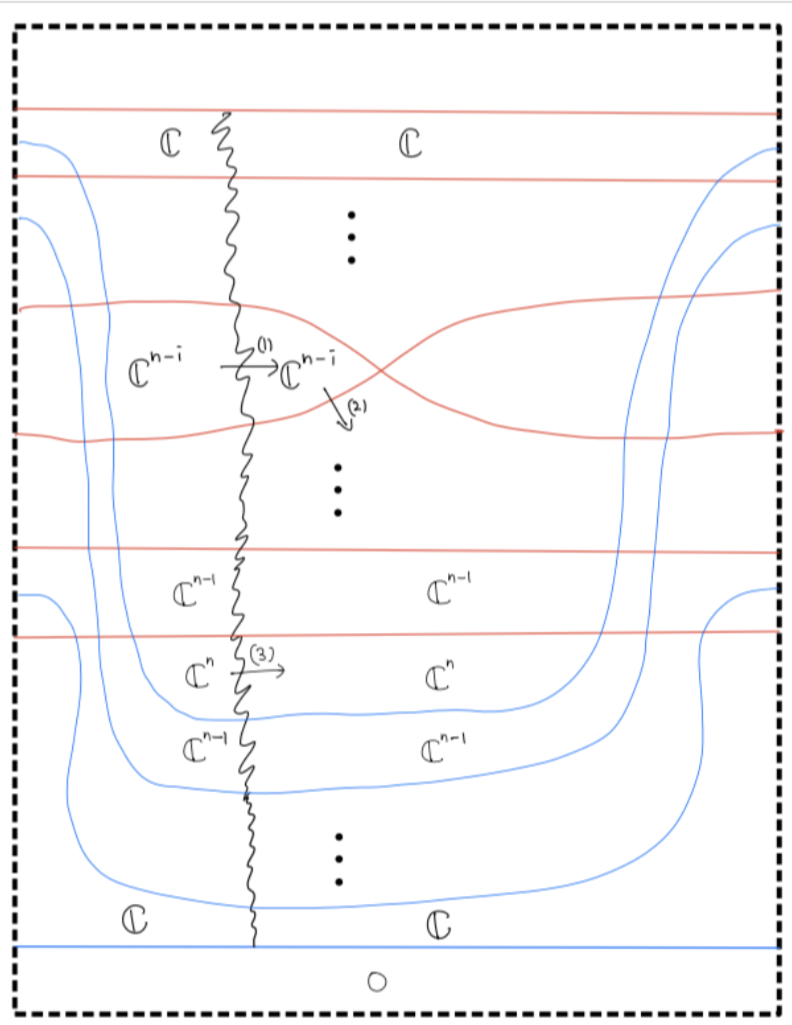
\includegraphics[scale = 0.95]{diagrams/cobord_gen/8.png}
    \caption{}
    \label{fig:your-label}
\end{figure}
\textbf{Generization maps}
\begin{enumerate}[label = (\arabic*)]
\item $diag(d_n,\cdots,d_{i+1})$
\item $\iota_0 \circ diag(1,\cdots,1) + e' I_{n-i+1,n-i}$
\item $diag(d_n,\cdots,d_1) + e I_{n-i+1,n-i}$
\end{enumerate}
\end{enumerate}
\pagebreak
\item If the generator $s_i$ is $i=1$,\\
\begin{enumerate}[label = (Step \arabic*)]
\item apply $cobord_{gen}(n-1)$ to the square region surrounded by purple dotted lines

\begin{figure}[H]
    \centering
    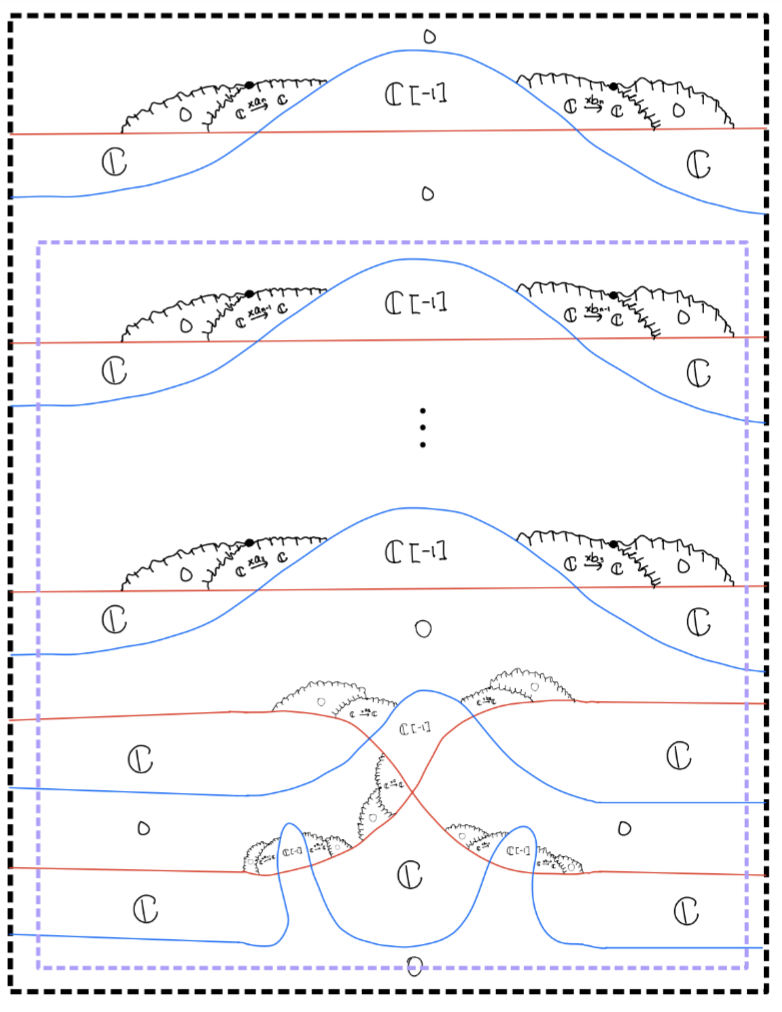
\includegraphics[scale = 0.95]{diagrams/cobord_gen/9.png}
    \caption{}
    \label{fig:your-label}
\end{figure}
\pagebreak
we get

\begin{figure}[H]
    \centering
    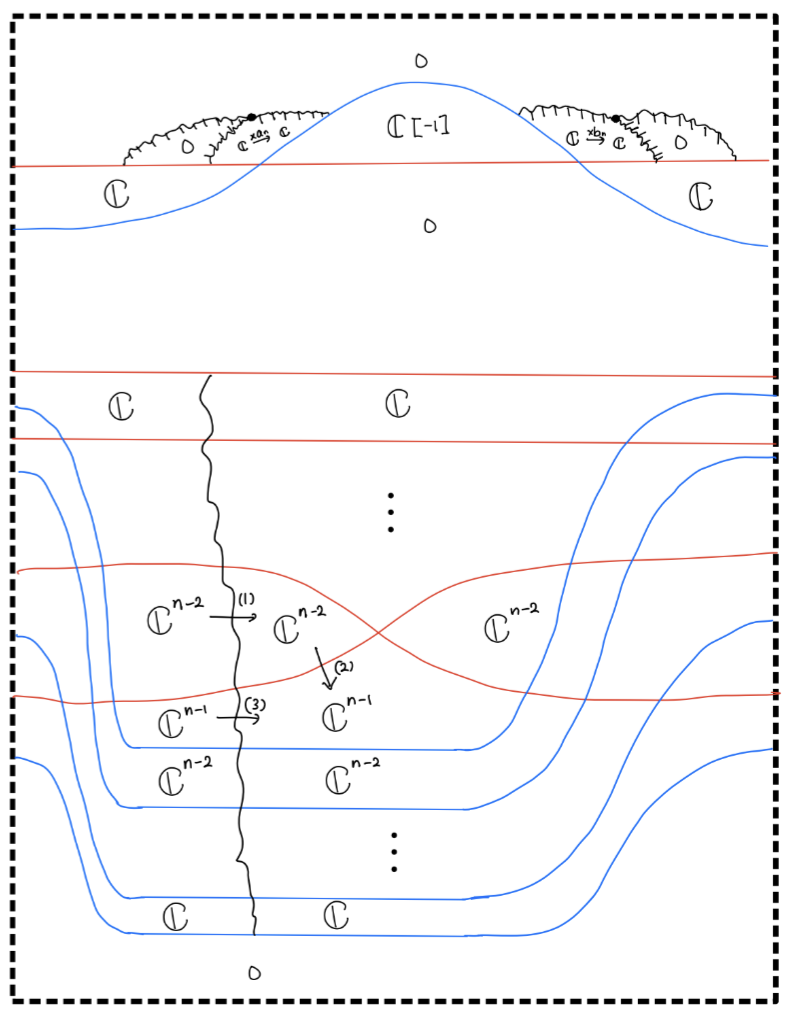
\includegraphics[scale = 0.95]{diagrams/cobord_gen/10.png}
    \caption{}
    \label{fig:your-label}
\end{figure}
\textbf{Generization maps}
\begin{enumerate}[label = (\arabic*)]
\item $diag(d_{n-1},\cdots,d_{2})$
\item $\iota_0 \circ diag(1,\cdots,1) + e' I_{n-1,n-2}$
\item $diag(d_{n-1},\cdots,d_1) + e I_{n-1,n-2}$
\end{enumerate}
\pagebreak
\item apply $cobord_2$ to the region surrounded by a purple dotted line

\begin{figure}[H]
    \centering
    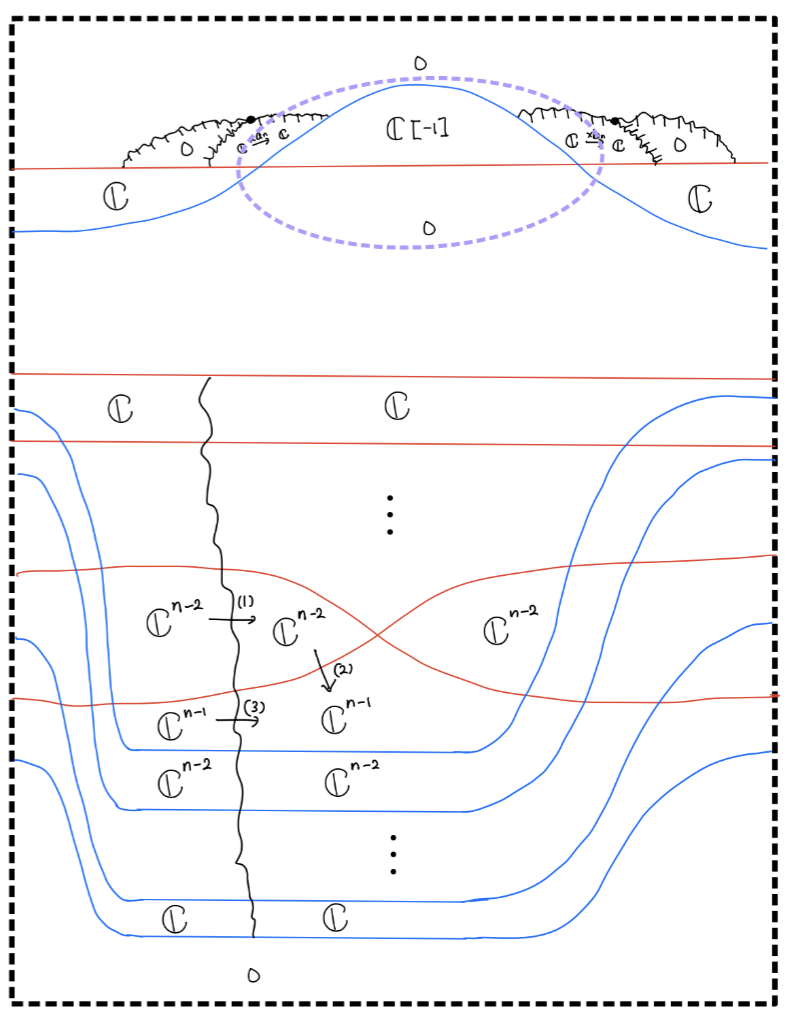
\includegraphics[scale = 0.95]{diagrams/cobord_gen/11.png}
    \caption{}
    \label{fig:your-label}
\end{figure}
\pagebreak
we get

\begin{figure}[H]
    \centering
    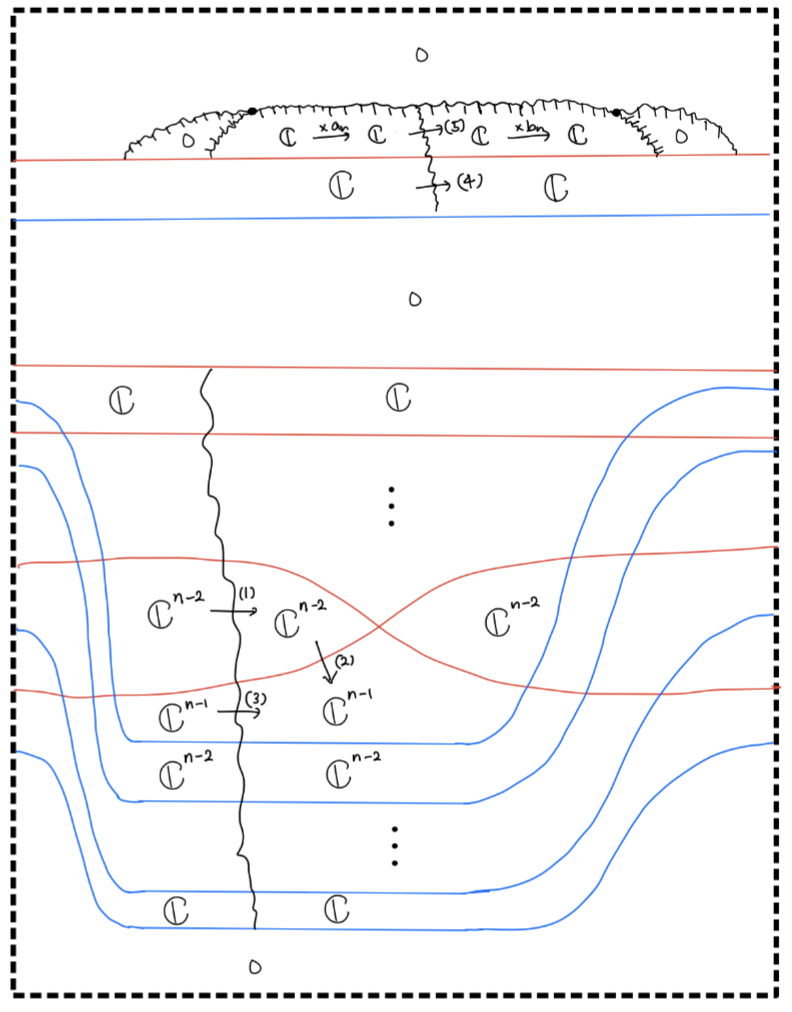
\includegraphics[scale = 0.95]{diagrams/cobord_gen/12.png}
    \caption{}
    \label{fig:your-label}
\end{figure}
\pagebreak
\textbf{Generization maps}
\begin{enumerate}[label = (\arabic*)]
\item $diag(d_{n-1},\cdots,d_{2})$
\item $\iota_0 \circ diag(1,\cdots,1) + e' I_{n-1,n-2}$
\item $diag(d_{n-1},\cdots,d_1) + e I_{n-1,n-2}$
\item $\times d_n$
\item 
\begin{tikzcd}
\C \arrow[r,"\times 1"] & \C \\
\C \arrow[r, "\times d_n"]\arrow[u,"\times d_n"] &\C \arrow[u,"\times b_n"]
\end{tikzcd}
\end{enumerate}
\pagebreak
which is quasi-isomorphic to 

\begin{figure}[H]
    \centering
    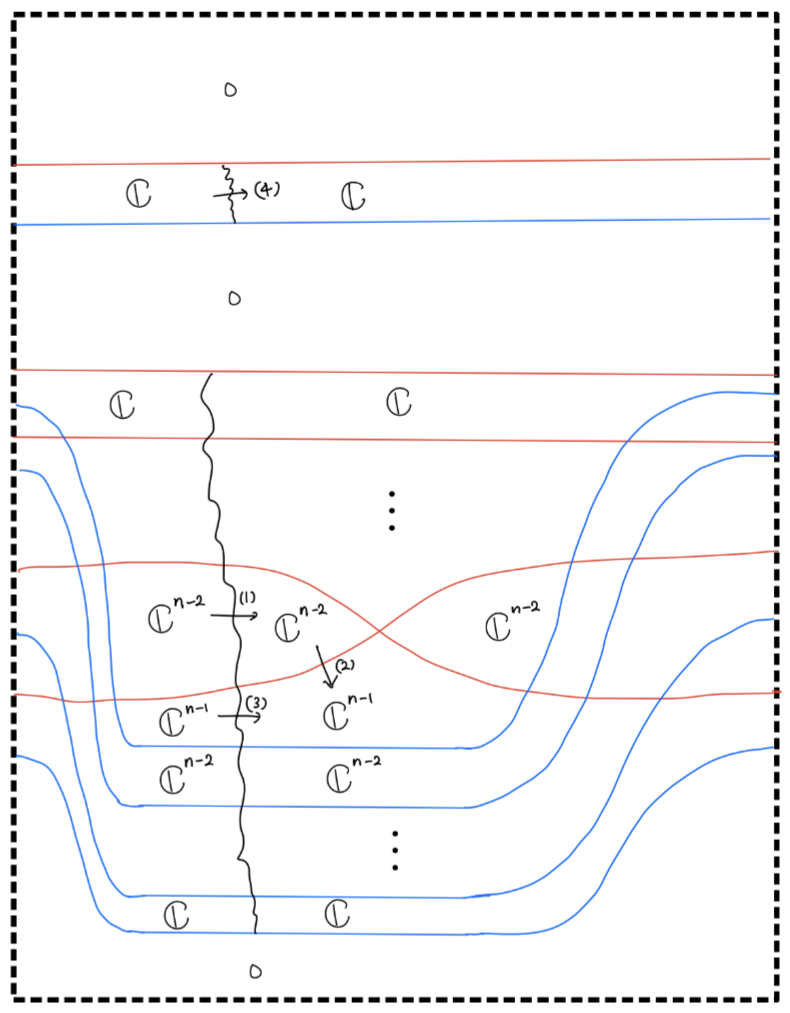
\includegraphics[scale = 0.85]{diagrams/cobord_gen/13.png}
    \caption{}
    \label{fig:your-label}
\end{figure}
\textbf{Generization maps}
\begin{enumerate}[label = (\arabic*)]
\item $diag(d_{n-1},\cdots,d_{2})$
\item $\iota_0 \circ diag(1,\cdots,1) + e' I_{n-1,n-2}$
\item $diag(d_{n-1},\cdots,d_1) + e I_{n-1,n-2}$
\item $\times d_n$
\end{enumerate}
\pagebreak
\item apply $cobord_5$ to the square region surrounded by purple dotted lines

\begin{figure}[H]
    \centering
    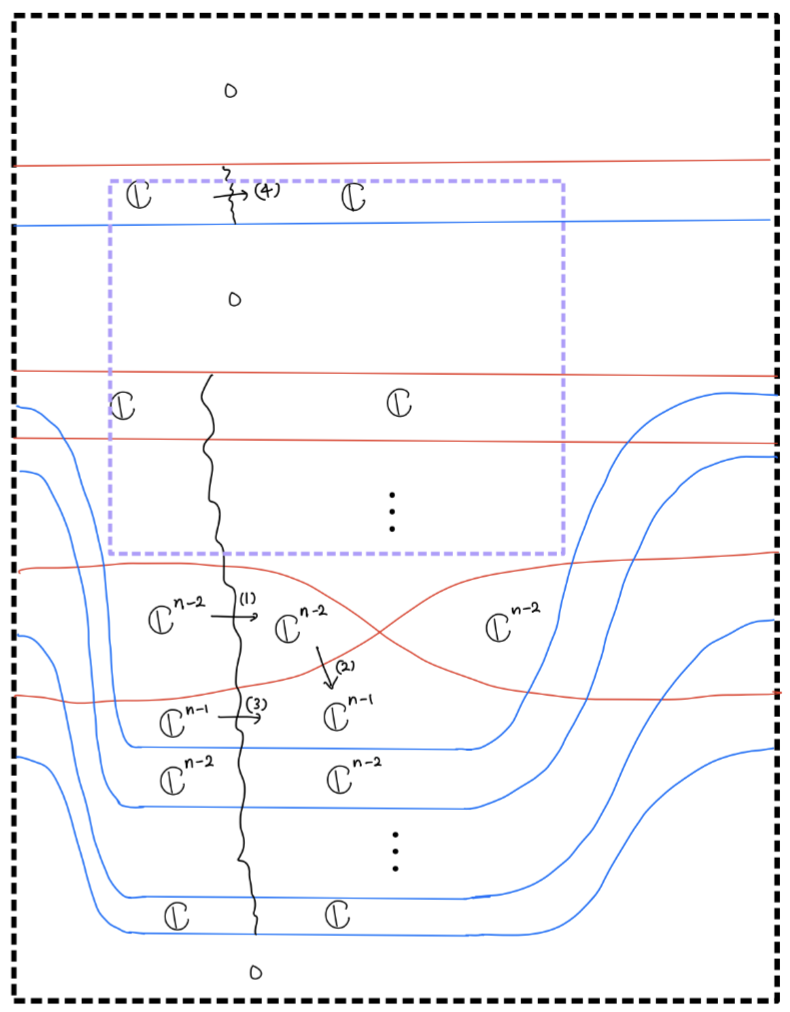
\includegraphics[scale = 0.95]{diagrams/cobord_gen/14.png}
    \caption{}
    \label{fig:your-label}
\end{figure}
\pagebreak
we get

\begin{figure}[H]
    \centering
    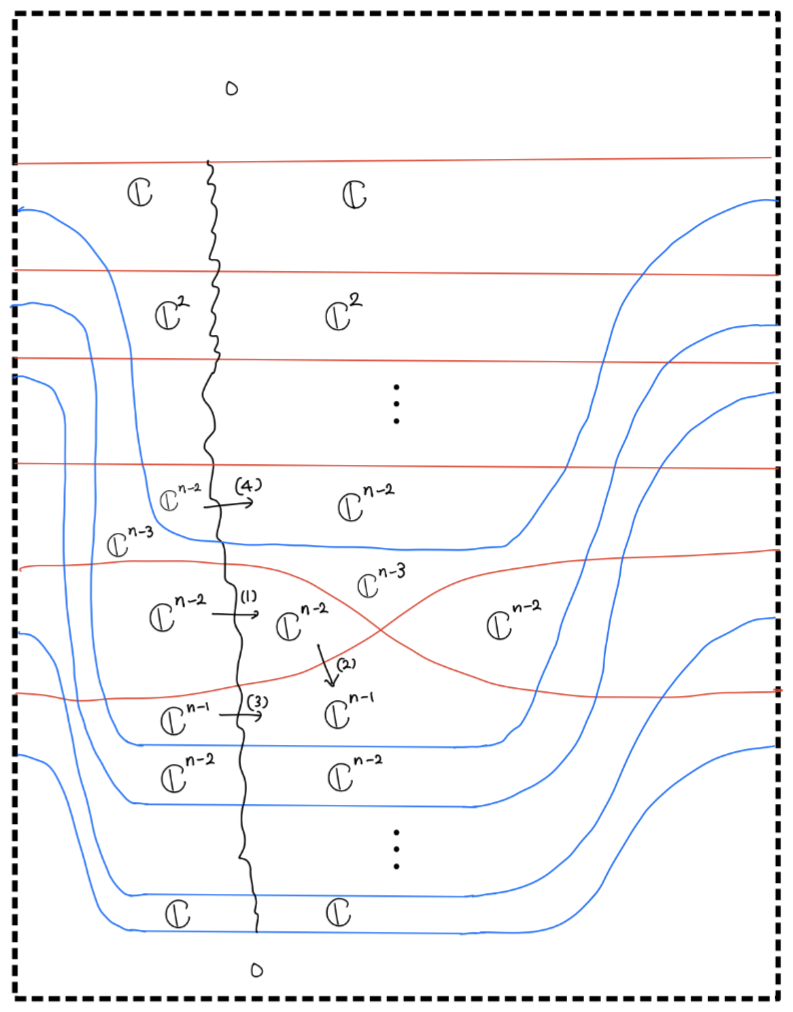
\includegraphics[scale = 0.85]{diagrams/cobord_gen/15.png}
    \caption{}
    \label{fig:your-label}
\end{figure}
\textbf{Generization maps}
\begin{enumerate}[label = (\arabic*)]
\item $diag(d_{n-1},\cdots,d_{2})$
\item $\iota_0 \circ diag(1,\cdots,1) + e' I_{n-1,n-2}$
\item $diag(d_{n-1},\cdots,d_1) + e I_{n-1,n-2}$
\item $diag(d_{n},\cdots,d_{3})$
\end{enumerate}
\pagebreak
\item apply $cobord_1$ to the regions surrounded by purple dotted lines

\begin{figure}[H]
    \centering
    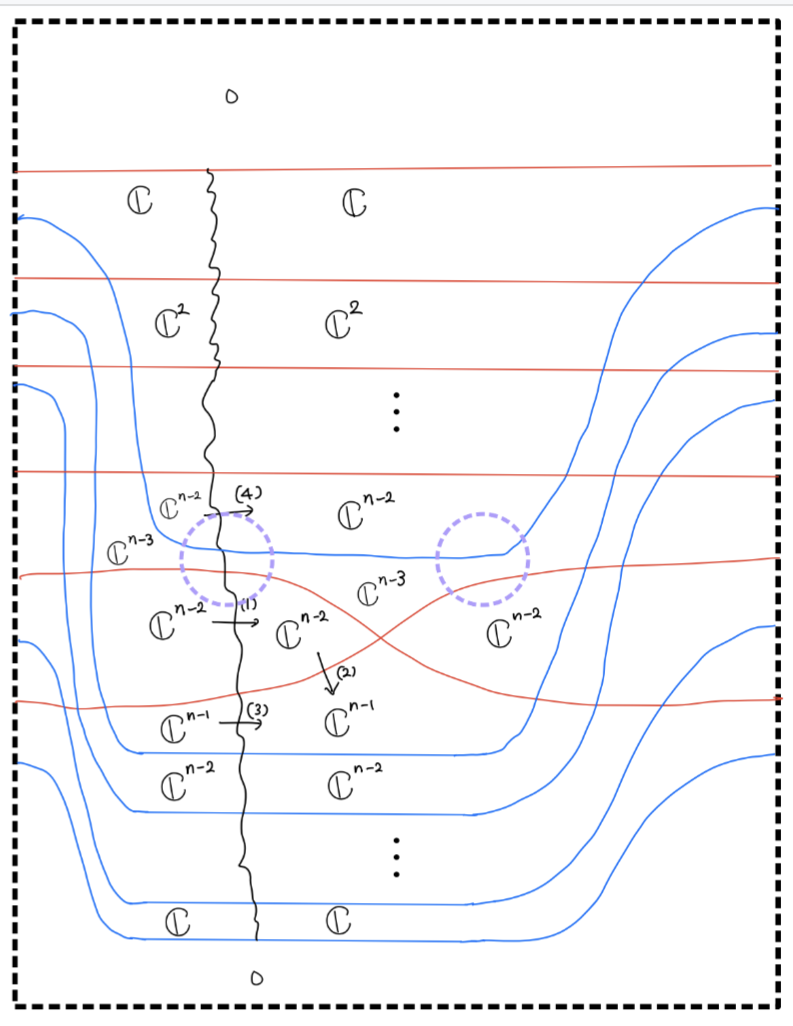
\includegraphics[scale = 0.95]{diagrams/cobord_gen/16.png}
    \caption{}
    \label{fig:your-label}
\end{figure}
\pagebreak
we get

\begin{figure}[H]
    \centering
    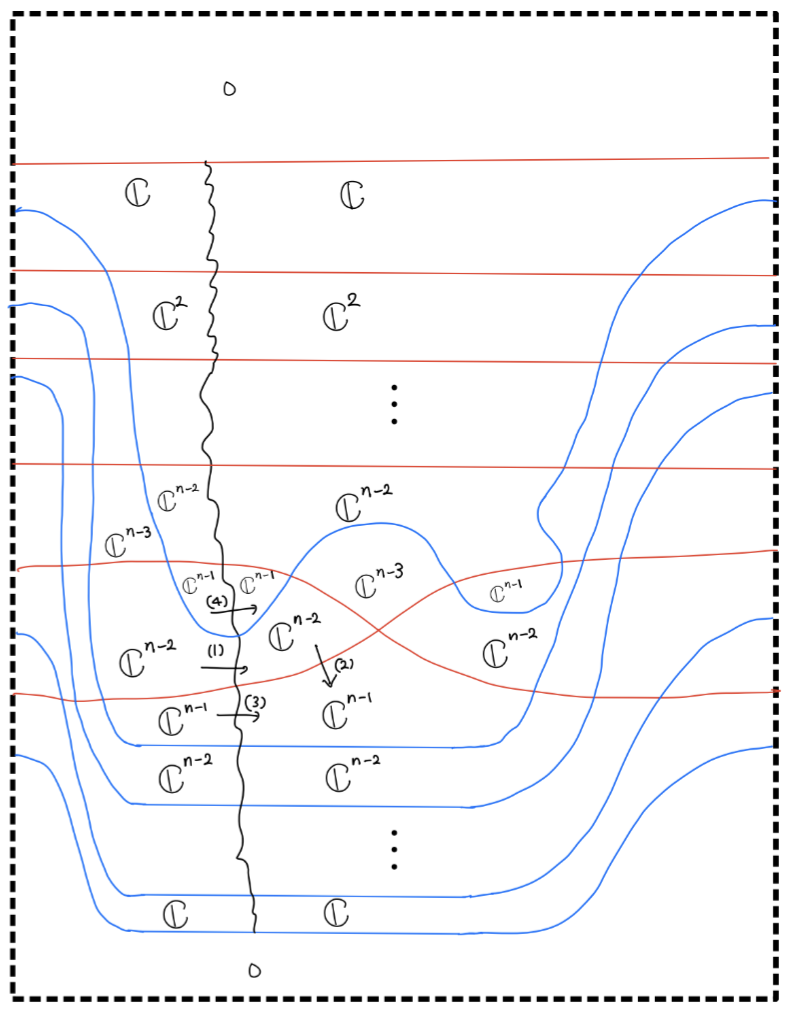
\includegraphics[scale = 0.85]{diagrams/cobord_gen/17.png}
    \caption{}
    \label{fig:your-label}
\end{figure}
\textbf{Generization maps}
\begin{enumerate}[label = (\arabic*)]
\item $diag(d_{n-1},\cdots,d_{2})$
\item $\iota_0 \circ diag(1,\cdots,1) + e' I_{n-1,n-2}$
\item $diag(d_{n-1},\cdots,d_1) + e I_{n-1,n-2}$
\item $diag(d_{n},\cdots,d_{2})$
\end{enumerate}

\pagebreak
\item apply $cobord'_8$ to the region surrounded by purple dotted lines

\begin{figure}[H]
    \centering
    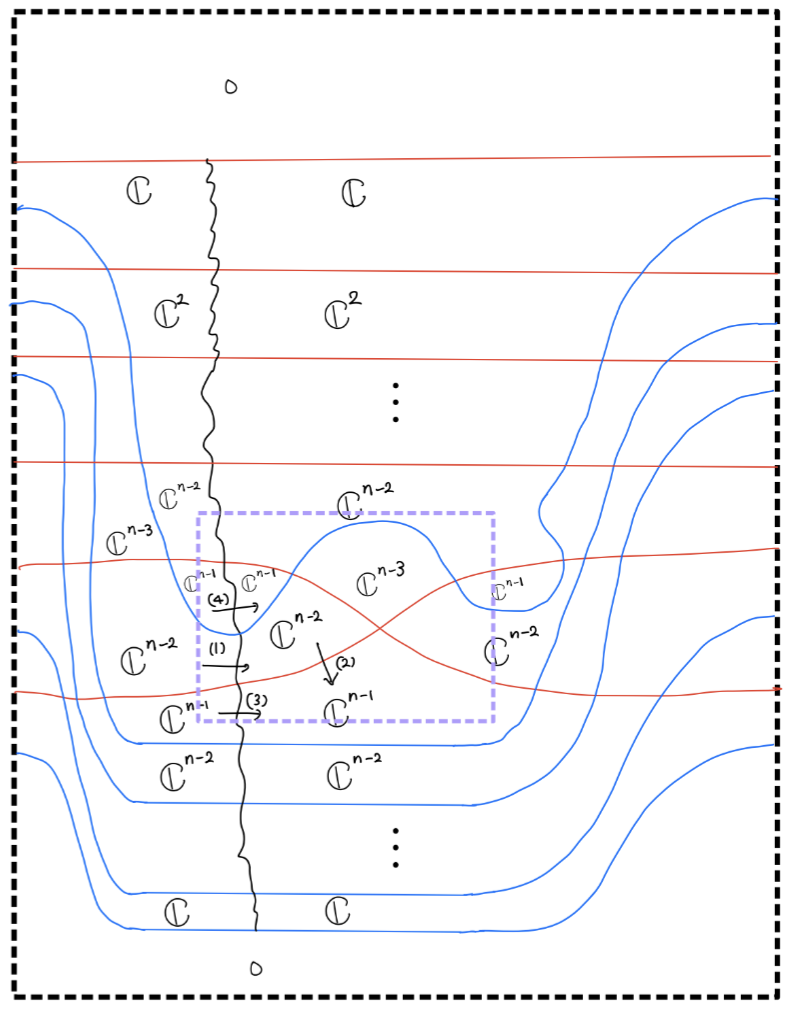
\includegraphics[scale = 0.95]{diagrams/cobord_gen/18.png}
    \caption{}
    \label{fig:your-label}
\end{figure}
\pagebreak
we get the final sheaf

\begin{figure}[H]
    \centering
    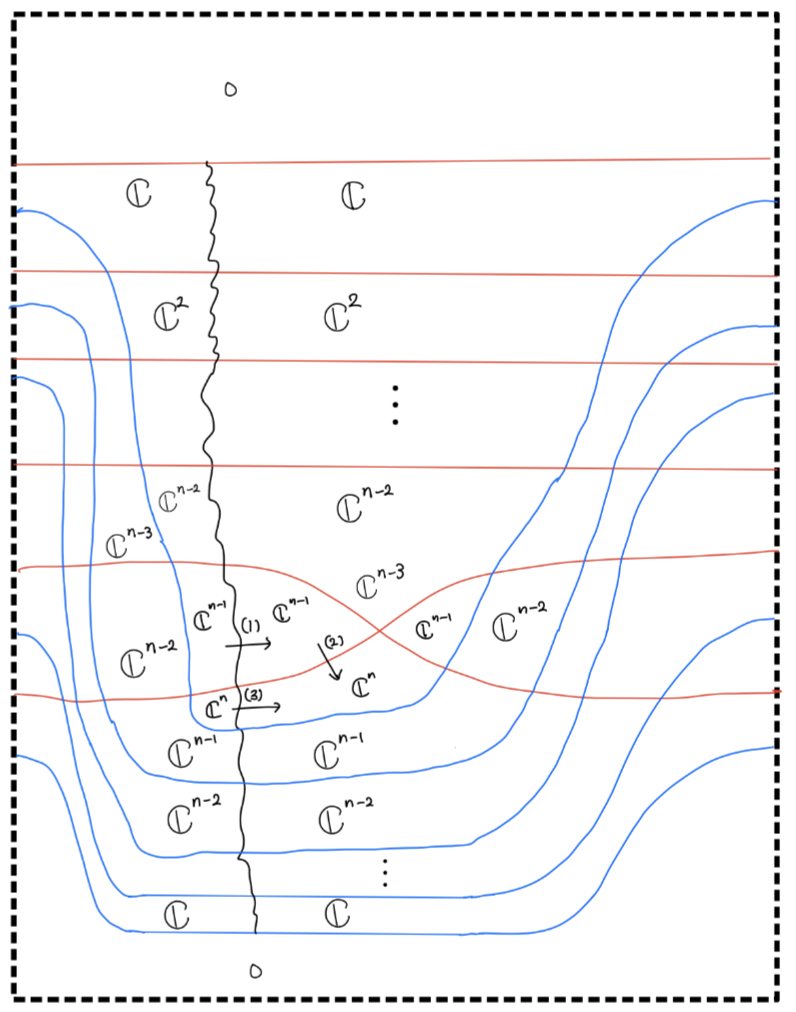
\includegraphics[scale = 0.95]{diagrams/cobord_gen/19.png}
    \caption{}
    \label{fig:your-label}
\end{figure}
\textbf{Generization maps}
\begin{enumerate}[label = (\arabic*)]
\item $diag(d_{n},\cdots,d_{2})$
\item $\iota_0 \circ diag(1,\cdots,1) + e' I_{n,n-1}$
\item $diag(d_{n},\cdots,d_1) + e I_{n,n-1}$
\end{enumerate}
\end{enumerate}
\end{enumerate}
\end{enumerate}
\pagebreak